\documentclass[11pt]{article}
\usepackage{geometry}                % See geometry.pdf to learn the layout options. There are lots.
\geometry{a4paper}                   % ... or a4paper or a5paper or ... 
%\geometry{landscape}                % Activate for for rotated page geometry
%\usepackage[parfill]{parskip}    % Activate to begin paragraphs with an empty line rather than an indent
\usepackage{graphicx}



%%Fonts
\usepackage[utf8]{inputenc}
\usepackage[english]{babel}
\usepackage[T1]{fontenc}
\usepackage{lmodern}

%% Maths
\usepackage{amsmath}
\usepackage{amssymb}
\usepackage{amsthm}
\usepackage{MnSymbol}
\usepackage{mathrsfs}
\usepackage{mathtools}
\usepackage{epstopdf}

%% Listings
\usepackage{listings}
\lstset{frame=tb, basicstyle=\ttfamily, language=Java, commentstyle=\color{red},
  keywordstyle=\color{blue}, numberstyle=\footnotesize,
basicstyle=\footnotesize}
\lstset{breaklines=true, breakatwhitespace=false}
\lstset{numbers=left, numberstyle=\scriptsize, firstnumber=1, columns=fullflexible, showstringspaces=false}

%% Other
\usepackage{enumerate}
\usepackage{paralist}
\usepackage{algpseudocode}
\usepackage{algorithm}
\usepackage{tikz}
\usetikzlibrary{positioning,shadows,arrows}
\usepackage{fancyvrb}
\usepackage{color}

\tikzset{
  treenode/.style = {align=center, inner sep=0pt, text centered,
    font=\sffamily},
  arn_n/.style = {treenode, circle, black, font=\sffamily, draw=black,
    fill=none, text width=1.5em}
}

%% Links
\usepackage{color}
\usepackage[pdfusetitle,pdftex,colorlinks]{hyperref}
\hypersetup{
    pdftitle={IS1350 Lab 1},
    pdfauthor={lkroll},
    pdfsubject={Operativsystem IS1350 Lab 1},
    pdfkeywords={},
    bookmarksnumbered=true,     
    bookmarksopen=true,         
    bookmarksopenlevel=1,       
    colorlinks=true,            
    pdfstartview=Fit,           
    pdfpagemode=UseOutlines,    % this is the option you were lookin for
    pdfpagelayout=TwoPageRight,
    urlcolor=blue
}

\DeclareGraphicsRule{.tif}{png}{.png}{`convert #1 `dirname #1`/`basename #1 .tif`.png}

%% COMMENTS %%
\newcommand{\TODO}[1]{\begingroup\def\thefootnote{\textcolor{red}{TODO}}\footnote{\textcolor{red}{#1}}\endgroup}
\newcommand{\TODOP}[1]{\par\textcolor{red}{#1}\marginpar{\textcolor{red}{TODO}}}
\newcommand{\TODOX}[1]{\textcolor{red}{#1}\marginpar{\textcolor{red}{TODO}}}

\newcommand {\N} {\mathbb{N}}
\newcommand {\Z} {\mathbb{Z}}
\newcommand {\R} {\mathbb{R}}
\newcommand {\C} {\mathbb{C}}
\newcommand {\Q} {\mathbb{Q}}
\newcommand {\Cx} {\mathcal{C}}
\newcommand {\strcon} {\squigarrowleftright}

\newcommand {\setofmaps} [2] {#2^#1}

\DeclareMathOperator{\Grad}{deg}
\DeclareMathOperator{\mini}{min}
\DeclareMathOperator{\cons}{cons}
\DeclareMathOperator{\nil}{nil}
\DeclareMathOperator{\true}{true}
\DeclareMathOperator{\false}{false}
\DeclareMathOperator{\tf}{tf}
\DeclareMathOperator{\idf}{idf}
\DeclareMathOperator{\tfidf}{tfidf}

\title{ID1020 -- Algorithms and Data Structures \\ Project 2 -- VT14 P2}
\author{}
\date{}                                           % Activate to display a given date or no date

\begin{document}
\maketitle
\section{Organisation}
The project is a programming task that is somewhat more challenging than the labs. You are expected to present your solution/code orally. We will assign grades to you based on the quality of your solution and your understanding of the involved concepts.\\

This is a description of \emph{Project 2 (P2)} which expands on \emph{Project 1 (P1)}.

\subsection{Dates}
\begin{description}
\item[Submission] Wednesday, Jan. 14th, 23:59 in Bilda
\item[Presentation] Thursday, Jan. 15th, time-slots will be assigned.
\end{description}

\subsection{Goals}
The project has the following goals:
\begin{itemize}
\item Work with the algorithms and data structures presented in the course
\item Reason about usage patterns in a software system and leverage this to make implementation decisions
\item Work on a real problem within the context of the course
\item Get an idea of CFGs and their ``real'' applications
\end{itemize}

\subsection{Requirements}
\label{ssec:reqs}
For the project you will need the following:
\begin{itemize}
\item Java
\item Maven
\end{itemize}
cf. Lab 2 for details.

\subsection{Time}
This depends heavily on your experience in writing code for more involved projects.\\
We can only recommend to start early, to get a feeling on how much time you will need to invest.\\
Make sure to think through the problem first before you throw yourself head first into coding. A good design from the beginning can save you many hours of wading through convoluted code later. 

\subsection{Notations \& Definitions}
\label{ssec:defs}
We denote the set of all natural numbers with $\N = \{1, 2, 3, 4, \ldots\}$ and $\N_0 = \{0\}\cup\N$. Similarly $\R$ denotes the set of all real numbers and $\R^+$ the set of all positive real numbers.\\
The set of common complexity classes is denoted as follows:
\begin{align*}
\Cx = \left\{f:\N\to\R \middle\mid f(n) \mapsto \left\{\begin{array}{l}1 \\ \log{n} \\ n \\ n\log{n} \\ n^r\mbox{ for some } r\in\R^+ \\ r^n \mbox{ for some } r\in\R^+ \\ n! \end{array}\right.\right\}
\end{align*}
Let $\setofmaps{\N}{\R}$ refer to the set of all functions $f:\N \to \R$ then clearly $\Cx \subseteq \setofmaps{\N}{\R}$.

\section{Background}
\label{sec:bg}
The goal of the project is to build a simple search engine for natural language text documents.\\
When completed the search engine will support the following operations:
\begin{itemize}
\item Index documents based on their content.
\item Find and list documents which contain a single provided key word.
\item Order search results by different properties (e.g. relevance, popularity).
\item Use a \emph{query language} to support more involved searches.
\end{itemize}

The documents themselves are provided in a specific format as part of the project framework and you don't have to worry about processing the raw files. However, it is important to notice that the given documents are english language texts of various types (e.g. short stories, newspaper articles, etc) and natural language texts differ in their treatment from more formal sources like programming languages, for example. The specific documents we provide are from the so called Brown Corpus\footnote{See \url{http://en.wikipedia.org/wiki/Brown_Corpus} for further reading, if you are interested.}. To give you some quick context, we provide a short summary of the field of natural language processing in section \ref{ssec:nlp}. Furthermore, the query language in the last task will require you to understand the concepts of parsing a limited syntax and to that end section \ref{ssec:cfg} introduces the concept of context-free grammars and their relationship with parsing syntax.

\subsection{Natural Language Processing}
\label{ssec:nlp}
Natural language processing (NLP) is a field of computer science, artificial intelligence, and linguistics concerned with the interactions between computers and human (natural) languages. To a large extent the purpose of NLP is to allow computers to derive and subsequently leverage information from documents written for and by humans. This information could be anything from simply observing word usage pattern in certain kinds of documents, to understanding and classifying the content of said documents on a semantic basis. NLP has a number of sub-fields of which the following might be of interest to our search engine:
\begin{description}
\item[Part-of-speech tagging] Given a sentence, determine the part of speech (POS) for each word. Many words, especially common ones, can serve as multiple parts of speech. For example, ``book'' can be a noun (``the book on the table'') or verb (``to book a flight''). Some languages have more such ambiguity than others. Languages with little inflectional morphology, such as English are particularly prone to such ambiguity. POS tagging is a necessary pre-requisite in most cases for any kind of syntactical analysis.
\item[Parsing] Determine the parse tree (grammatical analysis) of a given sentence. The grammar for natural languages is ambiguous and typical sentences have multiple possible analyses. In fact, perhaps surprisingly, for a typical sentence there may be thousands of potential parses (most of which will seem completely nonsensical to a human).
\item[Sentence breaking] (also known as sentence boundary disambiguation)\\
Given a chunk of text, find the sentence boundaries. Sentence boundaries are often marked by periods or other punctuation marks, but these same characters can serve other purposes (e.g. marking abbreviations).
\item[Word sense disambiguation]
Many words have more than one meaning; we have to select the meaning which makes the most sense in context. For this problem, we are typically given a list of words and associated word senses, e.g. from a dictionary or from an online resource such as WordNet.
\end{description}
If you are interested, \url{http://en.wikipedia.org/wiki/Natural_language_processing} give a good overview of the field.

\subsection{Context-free Grammars}
\label{ssec:cfg}
Context-free Grammars (CFGs) have their roots in formal language theory and were originally invented in an attempt to formalise the grammatical structure of natural languages. Since it has been shown that not all natural languages can be described by CFGs they have somewhat lost their importance in the NLP field. However, they retain immense importance in computer science as they form the basis of all programming languages (and also query languages, which is why we introduce them here).
\paragraph{Definition}
Formally a CFG is defined by a set of \emph{production rules} of the form:
\begin{equation*}
S \to s_1s_2\ldots s_n \mbox{ for } n\in\N_0
\end{equation*}
where $S$ is a \emph{nonterminal} symbol and the $s_i$ are either nonterminal or \emph{terminal}, meaning that $s_i$ is a \emph{token} of the alphabet of the language. Terminal symbols may never appear on the left-hand side of a production rule and each nonterminal symbol has to appear on at least one left-hand side of some production rule.

\paragraph{Example}
Consider the following grammar for simple arithmetical expressions:
\begin{align*}
1: E &\to num \mbox{ where } num\in\R \mbox{ for example} \\
2: E &\to E\cdot E \\
3: E &\to \frac{E}{E}\\
4: E &\to E+E \\
5: E &\to E-E \\
6: E &\to ( E )
\end{align*}
Also consider the following example sentence $s$ in the language of arithmetical expressions $s=2\cdot(3+4)$.

\paragraph{Definition}
In order to show that a sentence is part of the language of a CFG we have to find a \emph{derivation}, that starting with the start symbol and applying production rules to the right hand hand side, we arrive at the sentence.

\paragraph{Example}
For the grammar above and sentence $s$ the following would be a possible derivation:
\begin{align*}
& E & \mbox{ start symbol} \\
& E\cdot E & \mbox{ rule 2} \\
& num(2)\cdot E & \mbox{ rule 1} \\
& num(2)\cdot(E) & \mbox{ rule 6} \\
& num(2)\cdot(E+E) & \mbox{ rule 4} \\
& num(2)\cdot(num(3)+E) & \mbox{ rule 1} \\
& num(2)\cdot(num(3)+num(4)) & \mbox{ rule 1}
\end{align*}
Since we have derived $s$ from the start symbol we have shown that $s$ is part of the given grammar.

\paragraph{Definition}
While it is not difficult for a human to find a derivation that matches a sentence, a program would have try a (possibly large number) of different derivation until it by chance finds one that matches the input sentence. Since this is not feasible, programs usually apply the opposite process to derivation, which is called \emph{parsing}. The result of the parsing process is a \emph{parse tree} with the start symbol on top and the syntactical structure of the sentence represented in the structure of the tree. If parsing consumed all the symbols of a sentence that sentence is part of the language of the grammar.

\paragraph{Example}
The following is a possible parse tree for $s$:\\
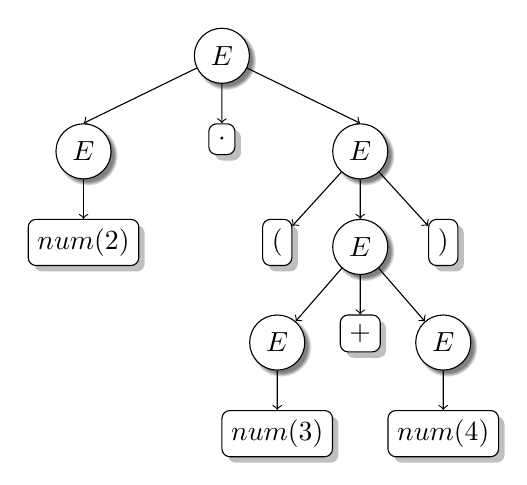
\begin{tikzpicture}[
    term/.style={rectangle, draw=black, rounded corners=1mm, fill=white, drop shadow,
        text centered, anchor=north, text=black},
    nonterm/.style={circle, draw=black, fill=white, circular drop shadow,
        text centered, anchor=north, text=black},
    level distance=0.5cm, growth parent anchor=south
]
\node (S0) [nonterm] {$E$} [->]
    [sibling distance=5em]
    child{ [sibling distance=2em]
    	node (S2) [nonterm] {$E$} [->]
	child{
		node (S4) [term] {$num(2)$}
	}
    }
    child {
    	node (S3) [term] {$\cdot$}
    }
    child{ [sibling distance=3em]
        node (S1) [nonterm] {$E$} [->]
        child{
		node (S6) [term] {$($}
	}
	child{
		node (S7) [nonterm] {$E$} [->]
		child{
			node (S9) [nonterm] {$E$} [->]
			child{
				node (S12) [term] {$num(3)$}
			}
		}
		child{
			node (S10) [term] {$+$}
		}
		child{
			node (S11) [nonterm] {$E$} [->]
			child{
				node (S13) [term] {$num(4)$}
			}
		}
	}
        child{
		node (S8) [term] {$)$}
	}
    }   
;
        
\end{tikzpicture}

\paragraph{Note} The quick introduction to CFGs presented here is certainly far from exhaustive. There are important issues of ambiguity and associativity of operations we have not considered at all so far. However, it should be sufficient to perform the required tasks. If you require more information or are simply interested feel free to look at \url{http://en.wikipedia.org/wiki/Context-free_grammar} and follow references from there.

\subsection{Notations}
\label{ssec:notations}
There are different types of notations used in logical/arithmetic  formulas.  In the next paragraphs we will discuss two of the notations which are relevant to our project.

\subparagraph{Infix Notation}
This is the most common notation where you have an operator in-between its operands for example: $3 + 5$ you have have an operator $+$ with two operands $3, 5$. 

\subparagraph{Prefix Notation}
In this notation you'll have the operator precedes the operands for example: $+ 3 \ 5$ which is equivalent to $3 + 5$ in \textit{infix notation}. A bit more complex example with nested expression :
\begin{verbatim}
+  -  3  5  +  4  9    is equivalent to    (3-5) + (4+9)
\end{verbatim}


\section{Helper Code}
In order for you to focus on implementing the tasks, we are supplying a Java code skeleton which contains the basic functionality for you to start coding. It encapsulates the reading and parsing of the pre-tagged words from the Brown Corpus (see section \ref{sec:bg}) and supplies sentence by sentence using a \textit{SentenceHandler} interface.\\

There are four main classes that you should know:
\begin{description}
\item[Word] encapsulates the word itself and the POS (verb, noun, adverb, etc)

\begin{lstlisting}
public class Word {
    public final PartOfSpeech pos;
    public final String word;
}
\end{lstlisting}

\item[Sentence] consists of a list of words

\begin{lstlisting}
public class Sentence {
    List<Word> words;
}
\end{lstlisting}

\item[Attributes] encapsulates the attributes that a word could have: a reference to the document in which the word was found and the occurrence (in number of preceding words) of the word in that document.
\begin{lstlisting}
public class Attributes {
    public final Document document;
    public final int occurrence;
}
\end{lstlisting}
\item[Document] contains the name of the document and the popularity (think ``number of views'').
\begin{lstlisting}
public class Document {
    public final String name;
    public final int popularity;
}
\end{lstlisting}
\end{description}

You are required to create your own \textit{TinySeachEngine} which implements the \textit{TinySearchEngineBase} interface.

\begin{lstlisting}
public interface TinySearchEngineBase {
    //Prepare to build the index
    public void preInserts();
    //Build the index
    public void insert(Sentence sentence, Attributes attr);
    //Finish up building the index
    public void postInserts();
    //Searching
    public List<Document> search(String query);
    //Convert Prefix into Infix
    public String infix(String query);
}
\end{lstlisting}

\paragraph{}
The two most important methods are:
\begin{description}
\item \textbf{insert:} adds the sentence with the given attribute to your index.
\item \textbf{search:} returns the list of documents that matches the query.
\end{description}
Additionally you have, \textbf{preInserts} and \textbf{postInserts} which you can use for setup purposes if you need to. Otherwise just leave the body of your implementation empty.\\
Lastly a new method \textbf{infix} is used to print an infix notation version of your search query. You should use this to double check that your parser interpreted the query correctly. So please use the same code as your parser does here. No copy\&paste; reuse your code! If you do not run exactly the same code, the method will be useless.

\subsection{Setup}
First you need to create a maven project and add our helper project as a dependency in your \textit{pom.xml} as follows:

\begin{lstlisting}[language=XML]

    <dependencies>
        <dependency>
            <groupId>se.kth.id1020</groupId>
            <artifactId>tinySearchEngine</artifactId>
            <version>2.0</version>
        </dependency>
    </dependencies>
    
    <repositories>
        <repository>
            <id>sics-release</id>
            <name>SICS Release Repository</name>
            <url>http://kompics.sics.se/maven/repository</url>
        </repository>
    </repositories>
    
\end{lstlisting}

In your main method you need to call \textit{Driver.run} which will starts reading the documents and will call \textit{insert} in turns to build the index, also it will start a  search REPL "read-eval-print-loop". To exit the REPL you can just write \textit{?exit} in front of search.

\begin{lstlisting}
    public static void main(String[] args) throws Exception{
        TinySearchEngineBase searchEngine = new TinySearchEngine();
        Driver.run(searchEngine);
    }
\end{lstlisting}

\paragraph{\textbf{Examples:}}
\begin{verbatim}
Building the index done in 1 seconds
Search: 
\end{verbatim}

As you can see first it prints that the indexing process is done in X seconds, and now on the next line you can enter your search query infront of search and hit enter for example, let's try to search for \textit{nightmare} and sort the result by popularity in an ascending order. 

\begin{verbatim}
Search: nightmare orderby popularity asc
Infix: nightmare orderby popularity asc
got 7 results in 157 microseconds
Document{cr04, pop=23661855}
Document{cp16, pop=314138678}
Document{ca04, pop=421696227}
Document{cl13, pop=728880313}
Document{cl23, pop=899544007}
Document{cc05, pop=1192381167}
Document{cf09, pop=1909872348}
Search: 
\end{verbatim}
 
\paragraph{Extra} If you want to go even further than using our helper project as a dependency and want to get a deep understanding and to start playing around with it, you can clone it from github \url{https://github.com/id1020/ht14-tinySearchEngine}.

\section{Query Language}
\label{sec:queries}

In this project we are going to optimize on the first project by extending the functionality of the query language.
We define a query language that should support prefix notation \ref{ssec:notations} which is more convenient  and simpler to parse. 

\subsection{Operators}
\label{ssec:operators}

The query language should support the following operators:
\begin{description}
\item \textbf{Intersection} \textbf{(+)} : returns all the documents containing both terms or more generally the intersection of both sub-queries results. 
\item \textbf{Union} \textbf{(|)}: returns all the documents that contain either one of the terms or more generally the union of  both sub-queries results.
\item \textbf{Difference} \textbf{(-)}: returns all the documents that contain the first term but not the second one, or more generally the set difference between the two sub-query results.
\item \textbf{Ordering} \textbf{(orderby)}: order the final result by the popularity of the document or by the relevance of the document to the query. We will discuss the relevance computation in detail in \ref{ssec:relevance}.
\end{description}


\paragraph{Formal Definition}  A more formal definition of the query language is described by the following CFG:
  
\begin{align*}
E &\to T &\mbox{ simple query}\\
E &\to T \ orderby \ Property \ Direction &\mbox{ ordering}\\
T &\to word &\mbox{ a search term} \\
T &\to + \ T \ T & \mbox{ intersection operation}  \\
T &\to | \ T \ T & \mbox{ union operation}  \\
T &\to - \ T \ T & \mbox{ set difference operation}  \\
Property &\to relevance &\mbox{ how relevant the document?}\\
Property &\to popularity &\mbox{ how popular is the document?}\\
Direction &\to asc &\mbox{ increasing order}\\
Direction &\to desc &\mbox{ decreasing order}
\end{align*}

According to our description of CFG in \ref{ssec:cfg}, In the above CFG, $E$ is a \textit{non-terminal} expression and $T$ could be \textit{terminal} or \textit{non-terminal}. $E$ is an expression consists of a set of tokens (words) that might end up by \textit{orderby Property Direction} or not which is described in the first two production rules above. Similarly, $T$ consists of a a single token or a set of tokens prefixed with an operator as described in the production rules above.

\paragraph{Note:} 
We replaced the ($T \to  \ T \ T$) rule from the first project with ($T \to \ |  \ T \ T$) which means that we don't support using the space as an operator. In other words, $T$ only consists of a single word also you can ignore the punctuation.

\paragraph{Examples: }

Let's have a more complex query that follows the query language described above. 

%+ + | nightmare stone | metaphysical stuck - + workbench night orderby popularity desc
\begin{footnotesize}
\begin{Verbatim}[commandchars=\\\{\}]
{\color{blue}+} {\color{blue}+} {\color{blue}|} nightmare stone {\color{blue}|} metaphysical stuck {\color{blue}-} dark night {\color{blue}orderby}  {\color{green}popularity}  {\color{blue}desc}
\end{Verbatim}
\end{footnotesize} 
Now let's try to convert this query from \textit{prefix notation} to \textit{infix notation} for clarity, first let's add parentheses for each operation we see in the query.

 \begin{footnotesize}
\begin{Verbatim}[commandchars=\\\{\}]
{\color{red}(}{\color{blue}+} {\color{red}(}{\color{blue}+} {\color{red}(}{\color{blue}|} nightmare stone{\color{red})} {\color{red}(}{\color{blue}|} metaphysical stuck{\color{red})}{\color{red})} {\color{red}(}{\color{blue}-} dark night{\color{red})}{\color{red})} {\color{blue}orderby}  {\color{green}popularity}  {\color{blue}desc}
\end{Verbatim}
\end{footnotesize} 

After adding the parentheses it became easy to convert it to \textit{infix notation} as shown below:

\begin{footnotesize}
\begin{Verbatim}[commandchars=\\\{\}]
{\color{red}(}{\color{red}(}{\color{red}(}nightmare {\color{blue}|} stone{\color{red})} {\color{blue}+} {\color{red}(}metaphysical {\color{blue}|}  stuck{\color{red})}{\color{red})} {\color{blue}+} {\color{red}(}dark {\color{blue}-} night{\color{red})}{\color{red})} {\color{blue}orderby}  {\color{green}popularity}  {\color{blue}desc}
\end{Verbatim}
\end{footnotesize} 
This example corresponds to the following parse-tree of the CFG:\\
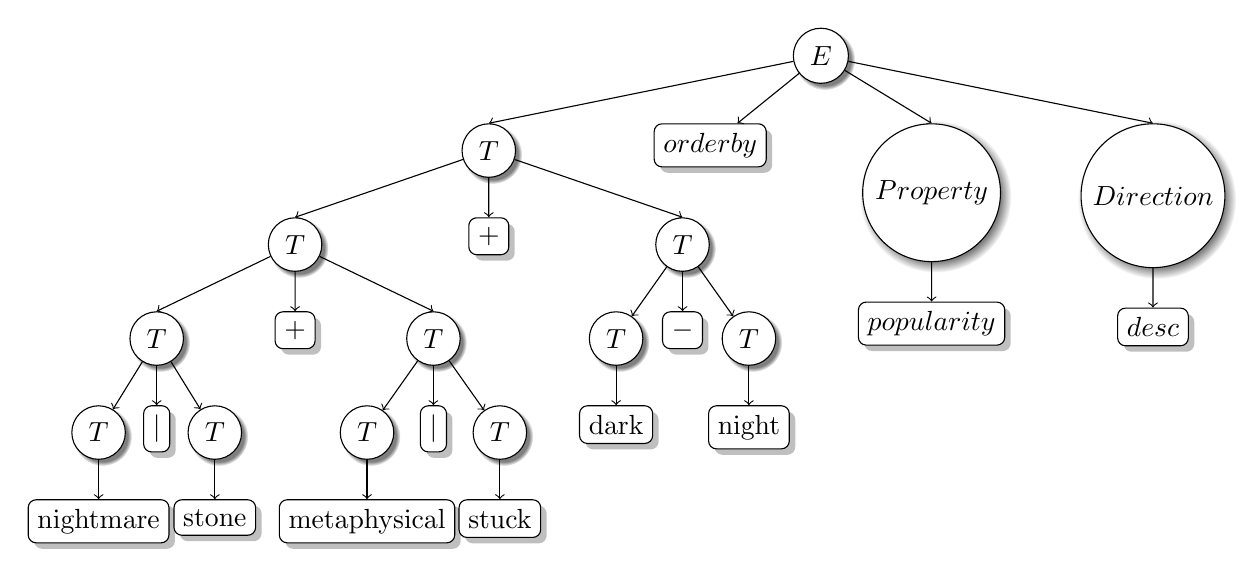
\begin{tikzpicture}[
    term/.style={rectangle, draw=black, rounded corners=1mm, fill=white, drop shadow,
        text centered, anchor=north, text=black},
    nonterm/.style={circle, draw=black, fill=white, circular drop shadow,
        text centered, anchor=north, text=black},
    level distance=0.5cm, growth parent anchor=south
]
\node (S0) [nonterm] {$E$} [->]
    [sibling distance=8em]
    child{ [sibling distance=7em]
    	node (S1) [nonterm] {$T$} [->]
	child{ [sibling distance=5em]
		node (S5) [nonterm] {$T$} [->]
		child { [sibling distance=2.1em]
			node (S10) [nonterm] {$T$} [->]
			child {
				node (S15) [nonterm] {$T$} [->]
				child {
					node (S24) [term] {nightmare}
				}
			}
			child {
				node (S16) [term] {$|$}
			}
			child {
				node (S17) [nonterm] {$T$} [->]
				child {
					node (S25) [term] {stone}
				}
			}
		}
		child {
			node (S11) [term] {$+$}
		}
		child { [sibling distance=2.4em]
			node (S12) [nonterm] {$T$} [->]
			child {
				node (S18) [nonterm] {$T$} [->]
				child {
					node (S26) [term] {metaphysical}
				}
			}
			child {
				node (S19) [term] {$|$}
			}
			child {
				node (S20) [nonterm] {$T$} [->]
				child {
					node (S27) [term] {stuck}
				}
			}
		}
	}
	child{
		node (S8) [term] {$+$}
	}
	child{ [sibling distance=2.4em]
		node (S9) [nonterm] {$T$} [->]
		child {
			node (S21) [nonterm] {$T$} [->]
			child {
				node (S28) [term] {dark}
			}
		}
		child {
			node (S13) [term] {$-$}
		}
		child {
			node (S23) [nonterm] {$T$} [->]
			child {
				node (S29) [term] {night}
			}
		}
	}
    }
    child {
    	node (S2) [term] {$orderby$}
    }
    child{ [sibling distance=3em]
        node (S3) [nonterm] {$Property$} [->]
        child {
        		node (S6) [term] {$popularity$}
        }
    } 
    child{ [sibling distance=3em]
        node (S4) [nonterm] {$Direction$} [->]
        child {
        		node (S7) [term] {$desc$}
        }  
    }  
;
        
\end{tikzpicture}\ \\

Let's try to analyze the query above by substituting sub queries with a named variable for simplicity and reference:
\begin{footnotesize}
\begin{Verbatim}[commandchars=\\\{\}]
A = {\color{red}(}nightmare {\color{blue}|} stone{\color{red})}
B = {\color{red}(}metaphysical {\color{blue}|}  stuck{\color{red})}
C = {\color{red}(}dark {\color{blue}-} night{\color{red})}

{\color{red}(}{\color{red}(} A {\color{blue}+} B {\color{red})} {\color{blue}+} C {\color{blue}orderby}  {\color{green}popularity}  {\color{blue}desc}
\end{Verbatim}
\end{footnotesize} 

\begin{description}
\item[A]  search for all documents that either contain \texttt{nightmare} or \texttt{stone}
\item[B]  search for all the documents that either contain \texttt{metaphysical} or \texttt{stuck} 
\item[C]  search for all the documents that contain \texttt{dark} but not \texttt{night}
\item[A+B+C] combine the results from \texttt{A} and \texttt{B} and \texttt{C}, that is all documents that contain either \texttt{nightmare} or \texttt{stone} and either \texttt{metaphysical} or \texttt{stuck} and \texttt{dark} but not \texttt{night}
\end{description}

By the running this query in your search engine, it should gives the following results:

\begin{footnotesize}
\begin{verbatim}
Search: + + | nightmare stone | metaphysical stuck - dark night orderby popularity desc
Infix: Query((((nightmare | stone) + (metaphysical | stuck)) + (dark - night)) ORDERBY POPULARITY DESC)
got 1 results in 0m 0s 36ms 955µs 160ns
Document{cn08, pop=1765493201}
\end{verbatim}
\end{footnotesize}

Another example by replacing the only \textbf{-} with \textbf{+} in the query, we got the following results:

\begin{footnotesize}
\begin{verbatim}
Search: + + | nightmare stone | metaphysical stuck + dark night orderby popularity desc
Infix: Query((((nightmare | stone) + (metaphysical | stuck)) + (dark + night)) ORDERBY POPULARITY DESC)
got 1 results in 0m 0s 1ms 425µs 62ns
Document{ck02, pop=453330457}
\end{verbatim}
\end{footnotesize}

\subsection{Relevance}
\label{ssec:relevance}
Previously in the first project, we used term frequencies to check relevancy of documents to the query. Now, let's consider a more meaningful metric \textit{\textbf{term frequency-inverse document frequency(tf-idf)}}. 

\begin{description}
\item[term frequency] measures how frequent the search term appears in the document. The more often, the more relevant.\\
It is given by $\tf(q, d)= \frac{n(q,d)}{T(d)}$ where $n(q,d)$ is how many times $q$ appeared in document $d$, and $T(d)$ is the total number of terms (words) in $d$.
\item[inverse document frequency] measures how often the search term appears in the index; whether the term is common or rare across all documents. The more often, the less relevant.\\
It is given by $\idf(q) = \log_{10}(\frac{N_D}{n_D(q)})$ where $N_D$ is the total number of documents, and $n_D(q)$ is the number of documents that contains $q$.
\end{description} 

Combing both equations, we get the tf-idf equation as follows:

\begin{equation}
\tfidf(q, d) = \tf(q, d) \cdot \idf(q) = \frac{n(q,d)}{T(d)} \cdot  \log_{10}(\frac{N_D}{n_D(q)})
\end{equation}

calculating the document relevance $\rho$ for a query $Q$ is just the sum of all underlying $\tfidf$ for each search term in the query
\begin{equation}
\rho(Q, d) = \sum_{q \in \tau(Q) }  \tfidf(q, d) \mbox{ with } \tau(Q) \mbox{ the set of search terms in } Q
\end{equation}

For example, if our query is \texttt{(+ nightmare stone)} then the relevance $\rho$ for a document $d$ would be

\begin{align*}
\rho&(\mbox{(+ nightmare stone)}, d) = \tfidf(\mbox{nightmare}, d) + \tfidf(\mbox{stone}, d) \\
&= \frac{n(\mbox{nightmare},d)}{T(d)} \cdot  \log_{10}(\frac{N_D}{n_D(\mbox{nightmare})}) + \frac{n(\mbox{stone},d)}{T(d)} \cdot  \log_{10}(\frac{N_D}{n_D(\mbox{stone})})
\end{align*}

\paragraph{Operators and Relevance:}
\begin{description}
\item[Intersection(+)] you should sum up the documents relevance of search terms, or more generally of sub queries.
\item[Union(|)] you should sum up the documents relevance of search terms, or more generally of sub queries.
\item[Difference(-)] you should consider only the relevance of the first operand.
\end{description}

\section{Tasks}

\subsection{Indexing -- 20P} 
\label{ssec:indexing}
Optimize upon the index building you did in the first project. You are allowed to use any data structure which you could feel it would improve your implementation. You are expected to analyse the time complexity of your chosen data structures/algorithms during the oral examination.\\

\subsection{Queries -- 50P} 
\begin{enumerate}
\item Implement the query language described in \ref{sec:queries}. \textbf{(25 P)}
\item Implement the relevance ordering described  in \ref{ssec:relevance}. \textbf{(15 P)}
\item Implement the \textit{infix} method  in \textit{TinySearchEngineBase} to convert from \textit{prefix notation} to \textit{infix notation}. \textbf{(10 P)}
\end{enumerate}

\paragraph{Tip} you could use Collections.sort for sorting your result query.

\subsection{Caching Sub-Queries - 30P}
In complex queries you'll end up by having a lot of nested sub-queries. In this task you are required to implement a simple caching mechanism to cache sub-queries results.  For example if the user searched for ({\color{blue}|} nightmare stone) and ({\color{blue}|} metaphysical stuck). If we cached the results for these two queries, it would be much faster to respond to this query ({\color{blue}+} {\color{blue}|} nightmare stone {\color{blue}|} metaphysical stuck).

\paragraph{Note:} In your cache you should consider the commutativity of (\textbf{+}) and (\textbf{|}) operations, for example ({\color{blue}|} metaphysical stuck) is the same as ({\color{blue}|} stuck metaphysical)
\label{ssec:caching}

\end{document}  